% !TeX spellcheck = en_US
\clearpage
\section{Experimental procedure and evaluation}
%
\subsection{Warning notices}\label{sec:warningnotices}
%
\begin{minipage}[c]{.15\linewidth}
	
\includegraphics[width=1.5cm]{img/toxic}
\end{minipage}
\begin{minipage}[t]{.85\linewidth}
	Eating and drinking is prohibited in the laboratory.
\end{minipage}\vspace{1em}\\ 
\begin{minipage}[c]{.15\linewidth}
	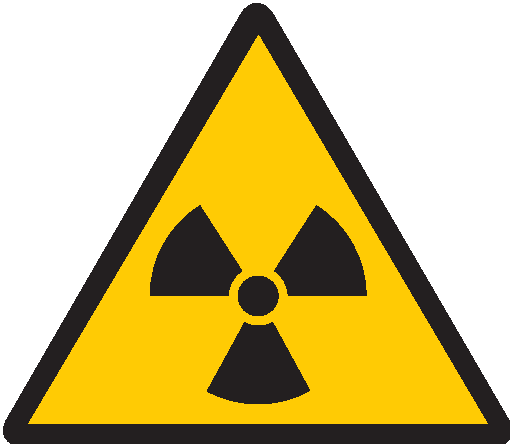
\includegraphics[width=1.5cm]{img/radioactive}
\end{minipage}
\begin{minipage}[t]{.85\linewidth}
	The radiation source used emits radioactive alpha radiation. It is weakly sealed and partially open. Radiation protection requires special safety measures for such sources. For this reason, the source has been permanently installed in the apparatus so that no radioactive material can escape from it into the room and no contact with the source is possible. Therefore, the measuring apparatus must not be opened under any circumstances. The ventilation valve should remain open for as short a time as possible.
\end{minipage}\vspace{1em}\\ 
\begin{minipage}[c]{.15\linewidth}
	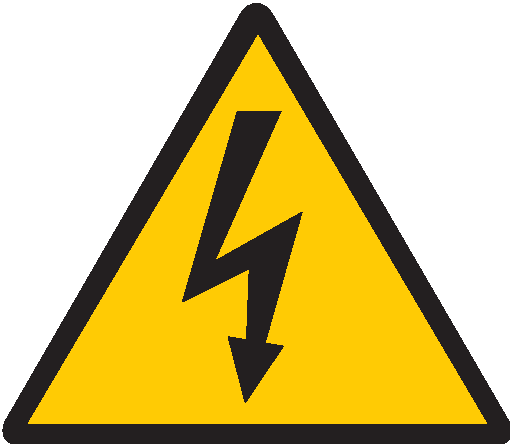
\includegraphics[width=1.5cm]{img/electric}
\end{minipage}
\begin{minipage}[t]{.85\linewidth}
	The maximum voltage on the semiconductor detector is $200$ V. Always change the voltage slowly. Exceeding the voltage can destroy the detector.
	\\ \\
	Only make changes to the wiring when the power supply is switched off.
	\\ \\
	The detector is extremely sensitive to light, operation with high voltage applied outside the closed vacuum chamber would destroy it.
\end{minipage}\vspace{1em}\\ 
\begin{minipage}[c]{.15\linewidth}
	
\includegraphics[width=1.5cm]{img/attention}
\end{minipage}
\begin{minipage}[t]{.85\linewidth}
	Do not open both venting valves of the vacuum piston at the same time.
	\\ \\
	Switch off the high voltage before venting.
\end{minipage}\vspace{1em}\\ 
%
\clearpage
%
\subsection{Preparations}
Go through this checklist together with the supervisor:
\begin{enumerate}
	\item Check the wiring (see Figure \ref{fig:verkabelung});
	\item Ensure that the power supply unit is set to $0$ V;
	\item Set the source to the smallest possible distance from the detector \\$r_{rel} = 0$ mm;
	\item Evacuate the vacuum chamber;
	\item Switch on Ortec-Crate;
	\item Start MCA3 Software on the PC.
\end{enumerate}
%
\subsection{Task 1: Saturation voltage}
The aim of the first task is to determine the saturation voltage of the semiconductor detector. The measurement is performed in vacuum at the smallest possible distance $r_{rel} = 0$ mm, and only for Plutonium.
\begin{enumerate}[label=\textbf{\alph*)}]
	\item At detector voltage $U_A = 0$ $V$, acquire a histogram with at least 8000 counts. Determine 
		\begin{itemize}[nosep]
		\item the peak position $\mu\ [\text{ADC Channels}]$;
		\item the half-width \textit{FWHM} [ADC Channels];
		\item and the counting rate $Z$ [1/s]
	\end{itemize}
	of the Plutonium peak using a Gaussian fit in the software.
	\item Repeat a) for the voltages $U_A = 8, 15, 20, 25, 30, 40, 70, 100$ V.
	\item Plot the peak position $\mu$, the count rate $Z$ and the percent resolution 
		\begin{equation}
			d_E = \frac{\textit{FWHM}}{\mu} \cdot 100 \qquad [\%]
		\end{equation}
	 as a function of $U_A$.
	\item Determine approximately the saturation voltage $U_{sat.}$ using the graphs. Select a voltage $U_{Det.}$ for your subsequent measurements. Explain your selection and the significance of the saturation voltage for using the semiconductor detector for $\alpha$-particle spectroscopy.
\end{enumerate}

\subsection{Task 2: Calibration and offset distance}
In this task, an energy calibration of the multi-channel analyzer is performed and the minimum adjustable distance $r_0$ (zero-distance) between detector and source is determined. The measurements take place in vacuum. 

\begin{enumerate}[label=\textbf{\alph*)}]
	\item Set the power supply voltage to the value $U_{Det.}$ determined in task 1;
	\item Record a reference spectrum with at least 12000 counts at $r_{rel} = 0$ mm.
		\\ Save a screenshot of the reference spectrum for your report.
		\\ \textit{Optional: } Save the histogram as a \texttt{.txt} file. This allows you to repeat the calibration at home.
	\item Calibrate the multi-channel analyzer in the software. To do this, determine the position of the three main maxima in the histogram by Gaussian fit and use the matching energies from Figure \ref{fig:schemata}. 
	
	Perform the Gaussian fits again to obtain the calibrated values for positions [keV], half-widths [keV] and count rates [1/s].
	\item Record at least 3000 counts at the relative distances $r_{rel} = 5, 10, 15, 20, 30$ mm and determine the calibrated positions, half-widths and count rates of the three main maxima by Gaussian fit.
	\item \textit{In the laboratory:} Plot the count rate as a function of the relative distance for Plutonium.
	
	\textit{In the report:} Plot the energy, percentage detector resolution and the counting-rate as a function of the relative distance for all isotopes.
	\item Determine the zero-distance $r_0$ between sample and detector in order to be able to use the effective distance $r_{eff} = r_0 + r_{rel}$ for the next measurements. To do this, consider how the distance law
	\begin{equation}
		Z \propto \frac{1}{r^2_{eff}},
	\end{equation}
	where $Z$ is the count rate in $[1/s]$, can be transformed and cleverly plotted to read the zero-distance directly from the y-axis intercept. Give the averaged result from the measurements of all three isotopes and present all values in a table.
 
    \textit{Note}: Looking at the error bars, decide wether to use the mean or the weighted mean with variance-defined weights to obtain the final result of $r_0$. See equation~\eqref{eq:weighted_mean} on page~\pageref{eq:weighted_mean} in the appendix.

\end{enumerate}
%
\subsection{Task 3: Range in air}
In the last part of the experiment, the differential energy loss of alpha radiation in air is determined.

\begin{enumerate}[label=\textbf{\alph*)}]
	\item Close the outlet valve of the vacuum chamber. Then slowly open the inlet valve until atmospheric pressure is established in the chamber. Then close the inlet valve again.
	\item Determine at $r_{rel} = 0, 4, 8, 20, 24, 28, 32, 36, \dots$ mm using a Gaussian fit:
	\begin{itemize}[nosep]
		\item the calibrated peak position $\mu\ [\text{keV}]$;
		\item the calibrated half-width \textit{FWHM} [keV];
		\item the count rate $Z$ [1/s];
	\end{itemize}
	for the main maxima of the three isotopes. If necessary, further increase the relative distance by $4$~mm per step until the plutonium signal disappears at $r_{max}$. Then take three additional measurements at $r_{rel} = r_{max} - 2, r_{max} - 6, r_{max} - 10$~mm. Record at least 2000 counts for each measurement.
	\item \textit{In the laboratory:} Plot the $\alpha$-energy $E\, \widehat{=}\, \mu$ depending on the effective distance for Plutonium. 
	
	\textit{In the report:} Plot the energy, the percentage resolution of the energy measurement, as well as the count rate depending on the effective distance for all three isotopes.
	\item Determine approximately -- by extrapolation with the eye -- the range of the $\alpha$-particles and their exit energy using the graph showing effective distance versus energy. What influences the uncertainty of the results the most?
	
	Compare the results with the literature values in a table. Use the given exit energies and Geiger's empirical range law, which gives the range $R$ [mm] depending on the exit energy $E_0$ [MeV] of the $\alpha$-particles:
	\begin{equation}\label{eq:geigerreachlaw}
		R = 3.1 \cdot \left(E_0\right)^{3/2}
	\end{equation}
	\textit{Optional:} If equation \ref{eq:geigerreachlaw} is transformed and adjusted accordingly, it is suitable as a fit function for the data. This allows range and exit energy to be determined more accurately than can be determined by eye.
	\item \textit{In the laboratory:} Plot the differential energy loss as a function of the effective distance $\left( \Delta E/ \Delta x \ \text{vs.}\ r_{eff} \right)$ for Plutonium.
	
	\textit{In the report:} Add the Bragg-Peaks of the other isotopes. Give an estimate of the maximum value of the energy loss and an estimate of the energy loss close to the sample. Compare the three Bragg curves with each other.
	\item Estimate the different contributions that go into the energy resolution. Consider the detector resolution from the vacuum and air measurements. Discuss the significance of the electronic noise, the statistical fluctuations in the number of electron-hole pairs (Fano factor), as well as the finite thickness of the source and the energy straggling.
\end{enumerate}

